\documentclass[12pt, a4paper, oneside]{amsart}
\setlength{\parindent}{0pt}
\usepackage[margin=2cm]{geometry}
\usepackage{amsmath}
\usepackage{amssymb}
\usepackage{amsfonts}
\usepackage[pdftex]{graphicx}
\usepackage[usenames]{color}
\usepackage{graphicx}
\usepackage{hyperref}
\usepackage{amsthm}

\title{Project 5: Text Manipulation on E-Mail Messages}
\author{Kevin Fujii and Erin Melcon}
\date{\today}

\begin{document}


\section*{Enron Email List}
The main purpose of this part of the project is to find all the email recipients and senders from the Enron data set, and summarize and graphically represent the results.  The first task was to extract the header of the emails, and then analyze the information.  This included looking for Bcc (Blind Carbon Copy) and Cc (Carbon Copy) fields.
\subsection*{Preliminary Investigations}
This was accomplished using regular expressions, and we found that if we do not include Bcc and Cc, we see that the person who emailed anyone the most was Jeff Dasovich.
\begin{table}[h]
\begin{center}
\begin{tabular}{|r|l|r|}
  \hline
Rank & Sender & Number of Emails \\ 
  \hline
1 & jeff.dasovich@enron.com & 131302 \\ 
2 & veronica.espinoza@enron.com & 110601 \\ 
3 & rhonda.denton@enron.com & 90730 \\ 
4 & cheryl.johnson@enron.com & 74632 \\ 
5 & jae.black@enron.com & 59196 \\ 
 \hline
\end{tabular}
\caption{The top 5 people who sent email from the Enron email list.}
\label{table:allLibs}
\end{center}
\end{table}
If we include Bcc and Ccs, the list remains the same.  We may now want to investigate who Jeff was emailing, and we at least two ways of doing that. The first is to build another frequency table, as follows:
\begin{table}[h]
\begin{center}
\begin{tabular}{|r|l|l|l|}
  \hline
Rank & Sender & Recipient & Frequency \\ 
  \hline
 1 & jeff.dasovich@enron.com & richard.shapiro@enron.com & 2909 \\ 
  2 & jeff.dasovich@enron.com & paul.kaufman@enron.com & 2768 \\ 
  3 & jeff.dasovich@enron.com & susan.mara@enron.com & 2746 \\ 
  4 & jeff.dasovich@enron.com & james.steffes@enron.com & 2725 \\ 
  5 & jeff.dasovich@enron.com & karen.denne@enron.com & 2489 \\ 
   \hline
\end{tabular}
\caption{The top five people that Jeff Dasovich emailed.}
\label{table:allLibs}
\end{center}
\end{table}
In which we can see the number of times Jeff emailed his top 5 recipients.  We may also look at a network graph;
\begin{figure}[htp]
\centering
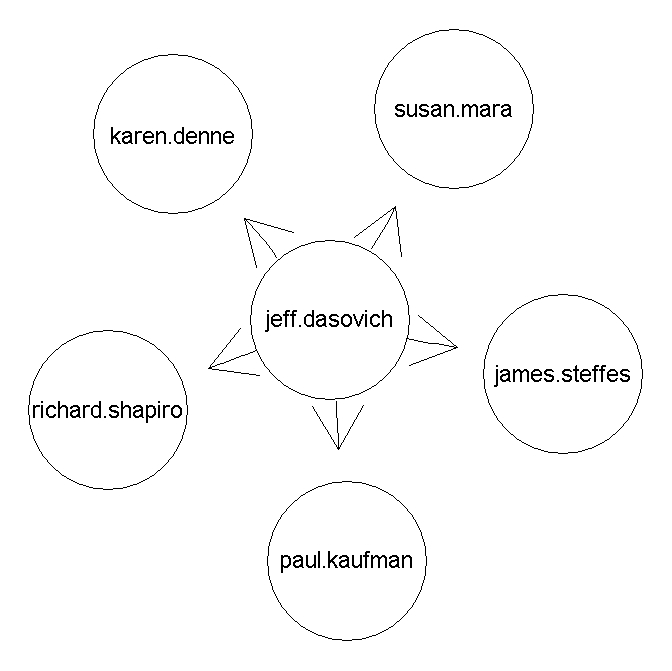
\includegraphics[width = 80mm]{JeffPlot.jpeg}
\caption{A small network of who Jeff emails}\label{fig:Small Jeff Network}
\end{figure}\\
Which gives us the same information, but visually, and without information about the weights.  However, with network graphs it is easy to see who people Jeff emailed were communicating with.  The following is a graph of the top three people Jeff was emailing, as well as the top three people his top three were emailing. 
\begin{figure}[htp]
\centering
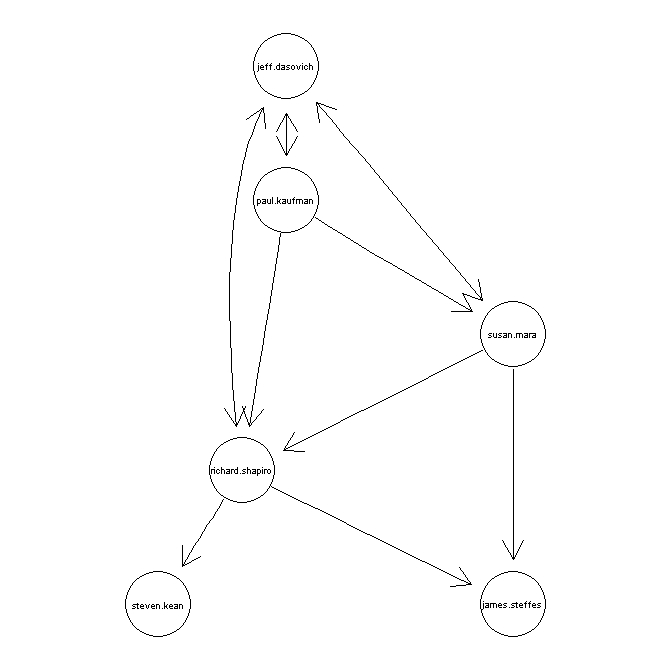
\includegraphics[width = 100mm]{JeffPlot2.jpeg}
\caption{A small network of who Jeff emails, and who they email.}\label{fig:Large Jeff Network}
\end{figure}\\
This shows that there is a small group, some of which email each other frequently. \\ 
\subsection{Who is Bccing?}
We may be interested in who is Bccing people, and who they are Bccing.  We find the following:
\begin{table}[ht]
\begin{center}
\begin{tabular}{|rlr|}
  \hline
 Rank & People & Frequency\\ 
  \hline
  1 & pete.davis@enron.com & 205896 \\ 
  2 & jeff.dasovich@enron.com & 24000 \\ 
  3 & vince.kaminski@enron.com & 19170 \\ 
  4 & kay.mann@enron.com & 13536 \\ 
  5 & kay.chapman@enron.com & 13530 \\ 
   \hline
\end{tabular}
\caption{The top five people that were Bccing.}
\label{table:allLibs}
\end{center}
\end{table}
It is interesting to see that Pete Davis Bcced a very large number of people.  In fact, if we look at all the emails grouped together (that is, disregarding if they were in the From, Bcc, or Cc field), we see
\begin{table}[ht]
\begin{center}
\begin{tabular}{|rlr|}
  \hline
 Rank & Sender & Frequency \\ 
  \hline
	1 & pete.davis@enron.com & 215046 \\ 
  2 & jeff.dasovich@enron.com & 155302 \\ 
  3 & veronica.espinoza@enron.com & 111745 \\ 
   \hline
\end{tabular}
\caption{The top three people that sent out any type of email.}
\label{table:allLibs}
\end{center}
\end{table}
that Pete sent out the most amount of emails as well.  Lets take a look at who Pete was emailing;
\begin{figure}[htp]
\centering
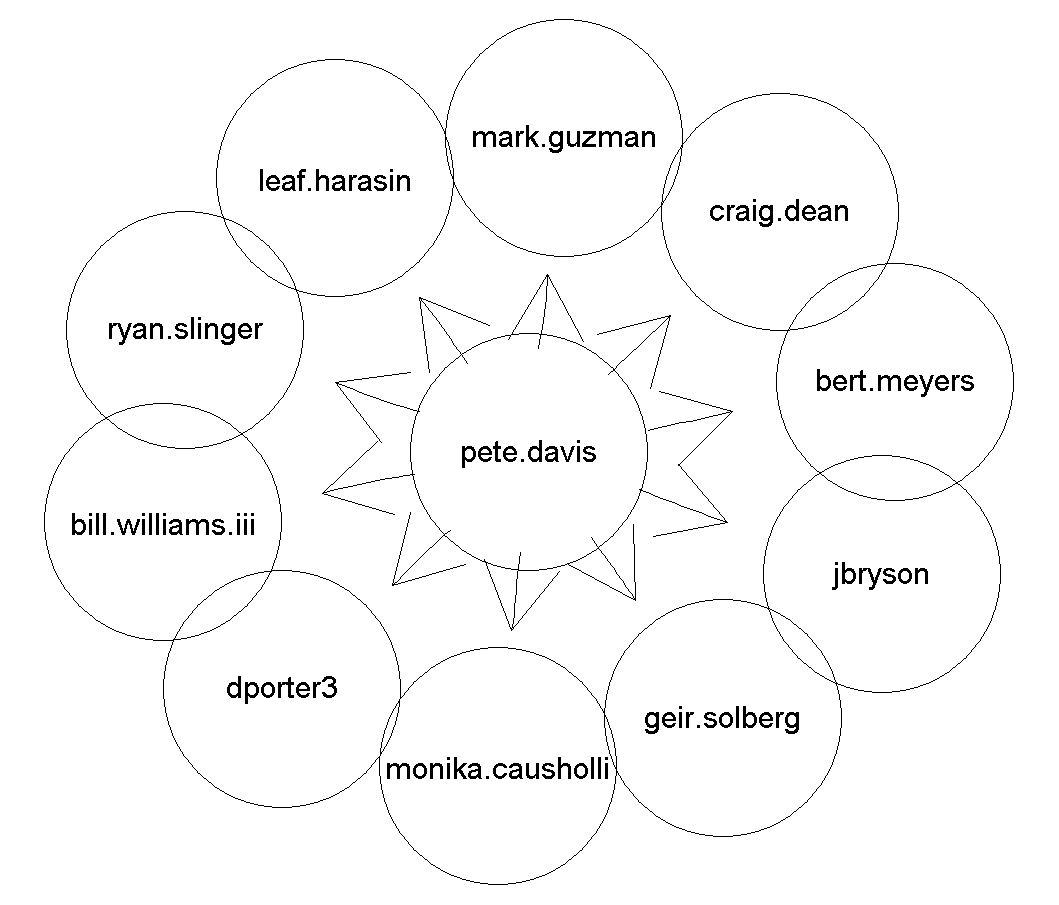
\includegraphics[width = 100mm]{PetePlot.jpeg}
\caption{A network of who Pete emails.}\label{fig:PeteNetwork}
\end{figure}\\

\end{document}